%%==============================================================
%% Modelo de TCC para o curso de Sistemas de Informação
%% da Universidade Federal de Viçosa - Campus de Rio Paranaíba
%% Autor: Rodrigo Smarzaro (smarzaro@ufv.br)
%% Última versão Agosto/2021
%% Arquivo em formato UTF-8
%% Compilar com pdftex e biber
%% Precisa do arquivo abntex2-UFV.sty
%%==============================================================

\documentclass[
    % -- opções da classe memoir --
    12pt,                   % tamanho da fonte
    openright,              % capítulos começam em página ímpar (insere página vazia caso preciso)
    oneside,                % para impressão só no anverso. Oposto a twoside
    a4paper,                % tamanho do papel.
    % -- opções do pacote abntex2 --
    % chapter=TITLE,        % Títulos em maiúsculas
    sumario=tradicional,    % Sumário padrão memoir 
    % -- opções do pacote babel --
    english,                % idioma adicional para hifenização
    brazil,                 % idioma principal do documento
    ]{abntex2}

% Pacotes fundamentais
\usepackage{abntex2-UFV}        % Personalização para a Universidade Federal de Viçosa
\usepackage{lmodern}            % Usa a fonte Latin Modern
\usepackage[T1]{fontenc}        % Seleção de códigos de fonte de saída
\usepackage[utf8]{inputenc}        % Codificação do documento (conversão automática dos acentos)
\usepackage{indentfirst}        % Indenta o primeiro parágrafo de cada seção.
\usepackage{graphicx}            % Inclusão de gráficos
\usepackage{booktabs}           % \toprule, \midrule e \bottomrule para tabelas
\usepackage{csquotes}
\usepackage[final]{microtype} 			% para melhorias de justificação
\usepackage{hyphenat}
\usepackage{nomencl}
\makenomenclature
\usepackage{float}

\usepackage{amsmath}




% Sistema autor-data com títulos nas referências em negrito
%\usepackage[alf,abnt-emphasize=bf]{abntex2cite}

% uso do biblatex, mais flexível e moderno
\usepackage[backend=biber,
            style=abnt,
            uniquename=init,
            giveninits,
            repeatfields,
            justify,
            noslsn]{biblatex}

\usepackage{xurl}
\urlstyle{same}

\addbibresource{referencias.bib}


% \PassOptionsToPackage{hyphens}{url}
% \usepackage{url}
% % permitir quebra de linha em URLs
% \makeatletter
% \g@addto@macro{\UrlBreaks}{\UrlOrds}
% \makeatother

% \setlength\bibparsep{10pt}

% ---
% CONFIGURAÇÕES DE PACOTES
% ---

% Informações de dados para CAPA e FOLHA DE ROSTO
\titulo{Georreferenciamento e classificação de árvores urbanas realizado por meio de imagens aéreas e aprendizado de máquina}
\autor{Paulo Roberto Ferreira Maciel}
\local{Rio Paranaíba}
\data{2026}
\orientador{Rodrigo Smarzaro}    % redefinido no abntex2-UFV para aceitar Instituição (default = UFV-CRP)
%\coorientador{Nome do Coorientador}
\instituicao{Universidade Federal de Viçosa}

\campus{\emph{Campus} Rio Paranaíba}      % pacote abntex2-UFV
\curso{Sistemas de Informação}               % pacote abntex2-UFV
\membrobancaA{Membro da Banca A}             % pacote abntex2-UFV default = UFV-CRP
\membrobancaB{Membro da Banca B}       % pacote abntex2-UFV default = UFV-CRP
\databanca{\today}                           % pacote abntex2-UFV

% O preambulo deve conter o tipo do trabalho, o objetivo,
% o nome da instituição e a área de concentração
\preambulo{Monografia apresentada à Universidade Federal de Viçosa, como parte das exigências para a a aprovação na disciplina Trabalho de Conclusão de Curso I}
% ---

% ---
% Configurações de aparência do PDF final

% informações para o arquivo pdf de saída
% Interessante alterar a cor dos links para preto(black)
% na versão final para imprimir
\makeatletter
\hypersetup{
        % metadados
        pdftitle={\@title},
        pdfauthor={\@author},
        pdfsubject={\imprimirpreambulo},
        pdfcreator={LaTeX with abnTeX2},
        colorlinks=true,   % false: links em frame; true: links coloridos
        linkcolor=black,   % cor dos links no documento
        citecolor=blue,    % cor dos links para a bibliografia
        filecolor=magenta, % cor dos links para arquivos
        urlcolor=blue,     % cor dos links para sites
        bookmarksdepth=4   % profundidade do sumário do PDF
}
\makeatother
% ---
%\usepackage{hyperref}
\begin{document}
% Retira espaço extra obsoleto entre as frases.
\frenchspacing

% ----------------------------------------------------------
% ELEMENTOS PRÉ-TEXTUAIS
% ----------------------------------------------------------
\pretextual

% Capa
\imprimircapa

% Folha de rosto
\imprimirfolhaderosto
% ---

% Inserir folha de aprovação
\imprimirfolhadeaprovacao



% Agradecimentos
\begin{agradecimentos}
%Insira o texto de agradecimentos aqui
    
    A Deus, por me fortalecer e me iluminar com sabedoria para a conclusão deste trabalho, e por sempre fazer parte da minha vida.
    
    Aos meus pais, irmãos, pelo apoio incondicional e por acreditar em mim o tempo todo.
    Aos meus amigos, pela paciência, compreensão e pelo incentivo durante a minha vida estudantil.

%posso colocar nomes de outros professores no agradecimento?
    Ao meu orientador, Professor Rodrigo Smarzaro, pelos conselhos, paciência e grandes contribuições ao desenvolvimento deste trabalho.
    Aos professores do curso, pelo ensino e apoio durante toda a formação.
    
    À Universidade Federal de Viçosa, pelos meios e pelo ambiente necessário para a realização deste trabalho.
    Ao instituto de tecnologia, pelo suporte técnico e infraestrutura.
    
    A todas as pessoas que de alguma forma ajudaram na realização deste trabalho, o meu sincero agradecimento.
    Aos colegas de curso, pelo companheirismo e pela troca de conhecimentos durante todos estes anos.

\end{agradecimentos}
% ---

% Epígrafe
\begin{epigrafe}
%“Find what you love and let it kill you.”

    \vspace*{\fill}
    \begin{flushright}
        \textit{``Podemos ver apenas um pouco à frente, mas podemos ver que há muito a ser feito.''\\
        (Alan Turing)}
    \end{flushright}
\end{epigrafe}
% ---

% RESUMOS

% resumo em português
\begin{resumo}
 \noindent
%Insira o resumo aqui
    Este artigo se concentra na aplicação de métodos de aprendizado de máquina e teledeteção para a identificação e classificação de espécies arbóreas. Durante a coleta de dados, VANTs serão utilizados para capturar imagens aéreas, enquanto um sistema de georreferenciamento baseado em GPS foi empregado no trajeto. As imagens de nível do solo serão capturadas e georreferenciadas por uma câmera de 360º, o que permitiu uma análise abrangente da área estudada. Para o treinamento dos modelos de aprendizado de máquina, foi criado um grande conjunto de dados, com amostras de campo, abrangendo imagens aéreas e do nível do solo. Diversos algoritmos de aprendizado de máquina, como Random Forest, SVM e Redes Neurais Convolucionais, serão analisados e comparados em termos de precisão na classificação de espécies arbóreas. Identificar espécies a partir de imagens de troncos e folhas é um grande desafio devido à alta variabilidade intraclasse e à semelhança entre classes. A variabilidade intraclasse está relacionada às grandes diferenças dentro de imagens de uma mesma espécie, causadas por fatores como variação de luz, ângulo de captura e o estado das árvores. A semelhança entre classes diz respeito à dificuldade de distinguir entre espécies diferentes apenas pela aparência. Problemas como balanço de cor inadequado nas câmeras podem resultar em tonalidades indesejadas, como o tom esverdeado, complicando ainda mais a classificação. Combinando técnicas de teledeteção, imagens aéreas e de solo, e algoritmos avançados de aprendizado de máquina, espera-se melhorar significativamente a precisão na classificação de espécies de árvores. Essa abordagem detalhada permite uma análise minuciosa das texturas dos troncos e das folhas, contribuindo para uma identificação mais precisa. Estudos anteriores, como os realizados por Kattenborn, Eichel e Fassnacht, mostraram que a segmentação com CNNs, como a U-net, pode alcançar até 84\% de precisão na classificação de vegetação usando imagens RGB de alta resolução espacial. A U-net tem se mostrado eficaz na segmentação de imagens, principalmente em cenários que exigem alta precisão e detalhamento, sendo capaz de capturar características complexas. A U-net tem demonstrado resultados consistentes em diversas aplicações de teledeteção e é considerada uma escolha confiável para projetos de análise de dados geoespaciais. A aplicação dessa técnica no projeto em questão poderá melhorar significativamente o desempenho na identificação e mapeamento de espécies arbóreas.
 \vspace{\onelineskip}

 \noindent
 \textbf{Palavras chaves}: Georeferenciamento, Open-Source Software, deep Learning, Imagens aéreas, Identificação e classificação automática de árvores, Sensoriamento Remoto, Algoritmos de Classificação, Segmentação de Imagens
\end{resumo}

% resumo em inglês
\begin{resumo}[Abstract]
\begin{otherlanguage*}{english}
   \noindent
    %Insira o abstract aqui
    This article focuses on the application of machine learning methods and remote sensing for the identification and classification of tree species. During data collection, UAVs were used to capture aerial images, while a GPS-based georeferencing system was employed along the route. Ground-level images were captured by a 360º camera, allowing for a comprehensive analysis of the studied area. A large dataset was created for training machine learning models, consisting of field samples that included both aerial and ground-level images. Various machine learning algorithms, such as Random Forest, SVM, and Convolutional Neural Networks, were analyzed and compared in terms of accuracy in tree species classification. Identifying species from images of trunks and leaves is a significant challenge due to high intraclass variability and interclass similarity. Intraclass variability refers to the substantial differences within images of the same species, caused by factors such as lighting variation, capture angle, and the condition of the trees. Interclass similarity refers to the difficulty of distinguishing between different species based solely on appearance. Issues such as improper color balance in cameras can result in unwanted hues, like a greenish tint, further complicating the classification process. By combining remote sensing techniques, aerial and ground images, and advanced machine learning algorithms, it is expected to significantly improve the accuracy of tree species classification. This detailed approach allows for a thorough analysis of trunk and leaf textures, contributing to more precise identification. Previous studies, such as those conducted by Kattenborn, Eichel, and Fassnacht, have shown that segmentation using CNNs, such as U-net, can achieve up to 84\% accuracy in vegetation classification using high spatial resolution RGB images. U-net has proven effective in image segmentation, especially in scenarios that demand high precision and detail, being capable of capturing complex features. U-net has demonstrated consistent results in various remote sensing applications and is considered a reliable choice for geospatial data analysis projects. Applying this technique to the current project could significantly enhance performance in identifying and mapping tree species.
   \vspace{\onelineskip}

   \noindent
   \textbf{Key words}: Georeferencing,
        Open-Source Software,
        deep Learning,
        Aerial Images,
        Automatic Tree Identification and Classification,
        Remote Sensing,
        Classification Algorithms,
        Image Segmentation
 \end{otherlanguage*}
\end{resumo}

% inserir lista de ilustrações
\pdfbookmark[0]{\listfigurename}{lof}
\listoffigures*
\cleardoublepage
% ---

% inserir lista de tabelas
\pdfbookmark[0]{\listtablename}{lot}
\listoftables*
\cleardoublepage
% ---

% Lista de siglas e abreviaturas (opcional)
% sintaxe: \item [sigla] Descrição da sigla

%\begin{siglas}
%\item[ABNT] Absurdas Normas Técnicas
%\item[UFV] Universidade Federal de Viçosa
%\item[CRP] \emph{Campus} de Rio Paranaíba
%\end{siglas}

% Lista de símbolos (opcional)
% sintaxe: \item [simbolo] Descrição do símbolo
\section*{Lista de Siglas e Abreviaturas}

\begin{description}
    \item[SR] Sensoriamento Remoto
    
    \item[IANS] Aerial imagens and ground level
    
    \item[6S] Second Simulation of the Satellite Signal in the Solar Spectrum
    
    \item[VANT] Unmanned Aerial Vehicles
    
    \item [SVM] \textit{support vector machine}
    
    \item [DEM] Modelos digitais de elevação
    
    \item [CNN] Redes neurais convolucionais
    
    \item  [GNSS] Sistema Global de Navegação por Satélite
    
    \item [SIG] Sistema de Informação Geográfico
    \item [QGIS] Quantum GIS
    
    \item [EO] \textit{electro-optics}
    
    \item[OSM] \textit{OpenStreetMap}
    
\end{description}
    
\newpage
 
%\begin{simbolos}
%\item[$\infty$ ] Infinito
%\end{simbolos}

% inserir o sumario
\pdfbookmark[0]{\contentsname}{toc}
\tableofcontents*
\cleardoublepage
% ---

% ----------------------------------------------------------
% ELEMENTOS TEXTUAIS
% ----------------------------------------------------------
\textual

%Modifique a estrutura dos capítulos e seções de acordo com a necessidade do seu trabalho
\chapter{Introdução}\label{sec:introducao}
% Contextualização do problema da detecção e identificação de árvores a partir de imagens aéreas e de rua
    No contexto urbano, o planejamento de áreas verdes tem se tornado uma prioridade para melhorar a qualidade de vida nas cidades, oferecendo benefícios como a mitigação das ilhas de calor, a melhoria da qualidade do ar e a promoção do bem-estar da população. A detecção e identificação de árvores a partir de imagens aéreas têm se mostrado uma ferramenta promissora para o monitoramento ambiental, o planejamento urbano e a conservação de áreas verdes \cite{herold2019role, f12121736}. No entanto, desafios como a dificuldade de classificar árvores em áreas densamente povoadas, a presença de sombras projetadas por edifícios e as condições adversas de iluminação em determinadas estações do ano indicam a necessidade de métodos adicionais que aprimorem a precisão dos resultados.

    Este trabalho visa desenvolver um sistema que integre imagens aéreas e de nível de rua, utilizando técnicas de visão computacional e aprendizado de máquina. A motivação central é incorporar as informações provenientes das imagens de nível de rua para melhorar a classificação das árvores que não puderam ser identificadas de maneira precisa apenas pelas imagens aéreas. Ao combinar essas diferentes perspectivas, o sistema proposto busca fornecer uma solução mais robusta e eficiente para o reconhecimento e a categorização de espécies arbóreas, auxiliando em estudos de ecologia, planejamento urbano e outras aplicações relacionadas à gestão sustentável dos recursos naturais.

    Este estudo possibilita a identificação eficiente de áreas carentes de arborização, permitindo a criação de políticas públicas mais precisas e orientadas ao planejamento sustentável das cidades.


% Justificativa da importância do estudo para a ecologia, planejamento urbano, monitoramento ambiental, etc.
    A importância dos estudos voltados para a detecção e identificação de árvores vai muito além do avanço técnico. Esses estudos são essenciais para uma variedade de campos, como ecologia, planejamento urbano e monitoramento ambiental, contribuindo significativamente para a gestão sustentável de recursos naturais e para o desenvolvimento de políticas públicas eficazes. Por exemplo, a necessidade de reduzir incertezas no mapeamento do uso da terra é crucial para a gestão de recursos hídricos, agricultura e florestas. Um exemplo claro é o investimento de 170 milhões de dólares pela Comissão Europeia em um sistema de contagem de árvores, destinado a registrar o número e as condições dessas árvores, fornecendo uma base para o controle e a gestão da ajuda financeira aos agricultores. Em áreas com características agronômicas complexas, abordagens que possam definir árvores individuais são especialmente necessárias para garantir uma gestão eficiente e eficaz dessas áreas \cite{daliakopoulos2009tree}.
    No contexto urbano, a importância das florestas urbanas não pode ser subestimada. Com o avanço rápido da urbanização, surgem desafios ambientais como poluição do ar, perda de espaços verdes e o efeito de ilhas de calor urbanas. As árvores urbanas desempenham um papel vital na regulação da temperatura, melhoria da qualidade do ar e na gestão dos ecossistemas urbanos. No entanto, a eficácia dessas funções depende diretamente da distribuição espacial e da variedade das espécies arbóreas. Portanto, a classificação precisa das espécies de árvores é essencial para o desenvolvimento sustentável das cidades. Técnicas tradicionais de classificação são laboriosas e ineficientes, levando à necessidade de abordagens mais modernas, como o sensoriamento remoto com UAVs (drones). A integração de múltiplas fontes de dados, como imagens RGB de alta resolução, LiDAR e dados hiperespectrais, tem mostrado um aumento significativo na precisão da classificação, chegando a 94,68\% de acurácia em estudos recentes \cite{wu2024fine}
    
    Além de sua importância para a ecologia e o planejamento urbano, a detecção precisa de árvores tem um papel crucial no gerenciamento de vegetação em áreas urbanas, especialmente na proximidade de redes elétricas. A poda preventiva de árvores é uma medida eficiente para reduzir os riscos de interrupções no fornecimento de energia, como rupturas de cabos, curtos-circuitos e incêndios, que podem ocorrer devido à interferência da vegetação com as linhas de distribuição elétrica urbana. Essas interferências são uma das principais causas de interrupções no fornecimento de energia, resultando em perdas financeiras significativas para as empresas de distribuição de energia devido à queda nos indicadores de qualidade e à necessidade de manutenção constante \cite{bergmann2024approach}. O uso de tecnologias como LiDAR e imagens esféricas, em combinação com métodos baseados em \textit{Deep Learning} (DL), pode automatizar a inspeção da vegetação, superando as limitações das imagens aéreas e reduzindo o tempo e o custo do monitoramento manual. Um estudo recente em quatro cidades brasileiras demonstrou que essa abordagem inovadora, implementada em uma plataforma web e aplicativo móvel, alcançou uma precisão superior a 94\% na identificação de interferências, mostrando seu potencial para aplicações em larga escala e contribuindo para a manutenção eficiente da rede elétrica.

    Esses avanços não apenas melhoram o gerenciamento das florestas urbanas e rurais, mas também contribuem para um planejamento mais consciente e eficiente em cidades que buscam mitigar os impactos ambientais da urbanização descontrolada. Assim, o estudo e a aplicação de tecnologias de sensoriamento remoto e visão computacional no contexto da detecção de árvores são fundamentais para a manutenção da saúde ambiental e o desenvolvimento sustentável das cidades e áreas rurais.

\chapter{Objetivos}\label{sec:objetivos}
%sugestão: 
  O objetivo geral deste projeto é desenvolver um sistema de detecção e classificação 
de árvores urbanas a partir de imagens aéreas de alta definição, capturadas por VANTs, 
com o apoio de algoritmos de processamento de imagens, visão computacional e aprendizado 
de máquina. O sistema foi aplicado na cidade de Rio Paranaíba -- MG, com foco na 
identificação automática de árvores em ambiente urbano.

\section{Objetivos Específicos}\label{sec:ObjetivosEspec}
%sugestão:
\begin{itemize}

\item Coletar imagens aéreas de alta definição da área urbana de Rio Paranaíba 
utilizando um VANT equipado com câmera RGB.

\item Desenvolver e treinar modelos de aprendizado de máquina baseados em Redes 
Neurais Convolucionais (CNNs) para a detecção de árvores nas imagens coletadas.

\item Implementar métodos de classificação que permitam identificar espécies arbóreas 
com base em características visuais extraídas das imagens aéreas, como forma, 
textura e cor das copas.

\item Avaliar o desempenho dos modelos por meio de métricas quantitativas, 
incluindo AUC, precisão e recall, utilizando conjuntos de dados de teste 
previamente rotulados.

\item Validar o sistema em cenário real de aplicação no monitoramento de 
áreas urbanas de Rio Paranaíba.

\end{itemize}

\chapter{Referencial Teórico}\label{sec:RefTeorico}
%Sugestão de Estrutura para o referencial teórico
    Para desenvolver sistemas que detectam e identificam árvores usando imagens aéreas e de solo, é essencial entender bem as tecnologias de sensoriamento remoto (SR), processamento de imagens e aprendizado de máquina. Nesta seção, exploramos os principais conceitos teóricos e os avanços tecnológicos que fundamentam este trabalho. Isso inclui o uso de satélites e drones para SR, técnicas de correção e pré-processamento de imagens, segmentação e classificação de objetos em visão computacional, além dos desafios específicos na detecção de árvores em ambientes variados. Também revisamos estudos anteriores que aplicaram essas tecnologias no mapeamento e monitoramento da vegetação, fornecendo uma base sólida para a implementação do sistema proposto.

\section{Sensoriamento Remoto e Imagens de Satélite}
% Conceitos básicos de sensoriamento remoto
    O SR é uma técnica sofisticada que possibilita a coleta de informações sobre a superfície terrestre sem a necessidade de contato direto. Isso é realizado por meio da captação da radiação solar que incide sobre a Terra ou da radiação eletromagnética artificial.\cite{figueiredo2005conceitos}.

    Os sensores envolvidos nesse processo são capazes de coletar uma gama diversificada de dados brutos, que incluem, mas não se limitam a, luz visível, infravermelho e micro-ondas, entre outras frequências. Após a coleta, esses dados são transmitidos via telemetria para estações terrestres.

    Nas estações terrestres, os dados são submetidos a processos de tratamento e armazenamento por meio de sistemas especializados. Isso permite que as informações coletadas sejam utilizadas de maneira eficaz para uma variedade de aplicações.

% Tipos de sensores utilizados em imagens de satélite (ópticos, SAR, etc.)
    Os sensores atuam de maneira semelhante às câmeras fotográficas, capturando ondas eletromagnéticas e as transformando em valores digitais ou pulsos eletrônicos. Esta transformação é realizada com base na intensidade da energia captada.

    Os sensores ópticos dependem da luz solar, pois captam a radiação eletromagnética refletida pela superfície da Terra. Por essa razão, esses sensores são denominados passivos. Eles são excelentes para a detecção de diferentes tipos de objetos devido às suas composições físico-químicas, textura e densidade \cite{figueiredo2005conceitos}.

    Em contrapartida, existem sensores que geram sua própria energia e funcionam na faixa de micro-ondas. Essa característica possibilita que eles operem tanto durante o dia quanto à noite, e em quaisquer condições climáticas. Essa é a principal vantagem dos sensores ativos \cite{florenzano2007iniciaccao}.

% Características das imagens de satélite (resolução espacial, espectral, temporal)

    A capacidade que o sensor tem de discriminar objetos em função do tamanho destes é chamada de resolução espacial. Nos sensores atuais, instalados em plataformas orbitais (satélites artificiais), esse tipo de resolução varia de 50 cm a 1 km. Um sensor com resolução espacial de 10 m, por exemplo, é capaz de detectar objetos maiores do que 100 m\textsuperscript{2}.

    A resolução espectral refere-se à capacidade de um sensor distinguir objetos com base em sua sensibilidade às diferentes partes do espectro eletromagnético. Sensores com faixas espectrais mais estreitas têm maior probabilidade de detectar pequenas variações na energia refletida. Além disso, um sensor com mais bandas ou canais tem uma resolução espectral superior, pois cada banda adicional oferece maior capacidade de discriminação espectral.

    A resolução temporal de um sensor refere-se à frequência com que ele captura imagens de uma determinada área. Por exemplo, o sensor TM-Landsat-5 tem uma resolução temporal de 16 dias, o que significa que ele captura imagens da mesma área a cada 16 dias. Isso é menos frequente, por exemplo, do que o sensor a bordo do satélite meteorológico Goes, que obtém imagens da mesma face da Terra a cada meia hora. Assim, a resolução temporal do sensor Goes é maior do que a do TM-Landsat-5 \cite{florenzano2007iniciaccao}.

% Aplicações de imagens de satélite na detecção de recursos naturais

    As imagens de satélite são ferramentas incríveis que ajudam em muitas áreas. Elas monitoram a vegetação, ajudando a proteger florestas e a criar políticas públicas eficazes. Além disso, identificam áreas com escassez de água, monitoram a qualidade da água e ajudam a prevenir a desertificação. Na agricultura, acompanham o crescimento das culturas, identificam problemas de irrigação e ajudam a prever a produção, tornando a gestão agrícola mais eficiente e sustentável. Essas imagens são essenciais para avaliar o impacto ambiental, analisando mudanças na cobertura da terra ao longo do tempo e monitorando atividades humanas. Elas também são vitais no gerenciamento de recursos, como em operações florestais e de mineração. \cite{geoinova2024, wu2024fine}.

\section{Tecnologias de Imagens de Drones}
   % Breve introdução aos drones e suas capacidades
    Um drone também chamados de Veículos Aéreos Não 
    Tripulados (VANTs), é uma aeronave operada sem um piloto humano a bordo, controlada autonomamente por computadores ou remotamente por um operador no solo\cite{Phang2023}. Sua capacidade de voar e manobrar é possibilitada por rotores ou hélices, permitindo manobras diversas. Equipados com sensores, câmeras e outras cargas úteis, os drones têm diversas funcionalidades, adaptando-se ao uso pretendido \cite{drones8040127}.

% Tipos de câmeras utilizadas em drones (RGB, multiespectral, térmica, NIR)
    Existem diversos tipos de câmeras utilizadas em drones, escolhidas conforme os objetivos e recursos disponíveis para o projeto em questão.

    A câmera RGB é um tipo de câmera que opera dentro do espectro visível. Ela é capaz de capturar imagens na faixa de luz que é visível a olho nu, sendo similar às câmeras convencionais encontradas em dispositivos como \textit{smartphones}.

    Esta câmera permite a obtenção de dados quantitativos do terreno. Com esses dados, é possível realizar análises detalhadas e gerar mapas topográficos. As análises podem incluir informações como coordenadas geográficas, distâncias, áreas, perímetros e outros aspectos relevantes.

    Uma câmera multiespectral é uma ferramenta sofisticada que adquire imagens em múltiplas bandas do espectro eletromagnético, que podem se estender além do alcance da luz visível até o infravermelho próximo (NIR). Após a captura, as imagens são analisadas permitindo a identificação precisa de áreas onde as plantas estão sofrendo estresse, bem como a detecção de deficiências nutricionais e outros problemas que podem afetar a saúde da planta. Além disso, as câmeras multiespectrais possuem a capacidade notável de detectar a presença de ervas daninhas e pragas, proporcionando uma visão abrangente da saúde do ecossistema observado \cite{droneng2024}.


    As câmeras térmicas detectam a temperatura de objetos e pessoas através da radiação infravermelha que emitem. Usando uma lente híbrida, combinam informações térmicas comuns para gerar imagens visíveis. São empregadas em segurança, detecção de incêndios, e medição de temperatura, podendo identificar múltiplas pessoas rapidamente, útil em cenários como a pandemia de COVID-19 \cite{aeon2024}.

    Os drones, com câmeras térmicas são uma ferramenta valiosa na agricultura e na pesquisa de vegetação. Identificam até características morfológicas e anatômicas das plantas, oferecendo assim dados experimentais mais precisos. Também detectam estresse hídrico, doenças e pragas antes que sejam visíveis, possibilitando ações preventivas pelos agricultores \cite{cnptia2024}.

   % Vantagens do uso de drones para captura de imagens em comparação com imagens de satélite
     Antes da popularização dos VANTs de pequena escala, o sensoriamento remoto próximo ao solo era realizado principalmente por aeronaves tripuladas equipadas com sensores multi-espectrais ou eletro-ópticos (EO). Essas missões, como a realizada em 1998 com um Cessna U206 para monitoramento de pragas e estresse em plantações de trigo, ofereciam alta resolução, mas eram operações caras e demoradas \cite{Phang2023}. Com o avanço dos VANTs (drones), uma alternativa mais acessível e ágil surgiu, permitindo a captura de imagens de alta resolução com maior frequência.
    
    No entanto, embora os drones ofereçam uma resolução espacial superior, especialmente para agricultura de precisão e monitoramento local, as imagens de satélite continuam a desempenhar um papel importante. As imagens de satélite possuem a vantagem de cobrir grandes áreas geográficas de uma só vez, o que é ideal para monitoramento de larga escala. Contudo, elas apresentam limitações em termos de resolução espacial em comparação com os drones. Os satélites, embora acessíveis para certos tipos de monitoramento, podem não fornecer o nível de detalhe necessário para aplicações que exigem uma análise mais refinada, como a identificação precisa de pequenas variações no campo.

    Os drones têm desempenhado um papel importante na melhoria da resolução de imagem usada na agricultura de precisão. Devido ao seu voo mais baixo e sobrevoos mais próximos da superfície do solo em comparação com a aeronave tripulada, os drones capturam mais detalhes das plantações e, portanto, oferecem melhor resolução para a condição da cultura e do solo. Isso os torna instrumentos muito úteis na otimização da gestão da ambiental e suporte à decisão informado \cite{Phang2023}.
    
    Embora os drones ofereçam uma resolução significativamente melhorada em comparação com aeronaves tripuladas, permitindo a captura de detalhes mais precisos das plantações e do solo, o uso dessa tecnologia em ambientes complexos, como áreas arborizadas ou urbanas, apresenta desafios específicos. A qualidade e a resolução das imagens capturadas nem sempre são suficientes para superar as dificuldades associadas à detecção de árvores em diferentes estágios de crescimento ou em cenários com sombras e obstruções.

   % Limitações e desafios do uso de drones para a detecção de árvores
    A pesquisa conduzida por \textcite{neto2012detecccao} destacou três desafios significativos na detecção de árvores utilizando drones. A variação do tamanho das copas e das alturas das árvores, a sombra dos edifícios sobre as árvores e a influência da estação do ano são fatores que complicam o uso dessa tecnologia. A variação da copa é um problema, pois uma árvore recém-plantada não apresenta uma copa bem definida, dificultando sua detecção. Além disso, edifícios e montanhas podem interferir no processo de eliminação de sombras, sobrepondo algumas árvores que acabam sendo eliminadas erroneamente.
    

\section{Processamento de Imagens e Visão Computacional}
   % Conceitos básicos de processamento de imagens
    No contexto das imagens de satélite, o vasto volume de dados e a complexidade dos cálculos demandam, de fato, recursos computacionais significativos. O processamento digital tornou-se uma área de grande investimento devido à alta demanda, e isso é particularmente verdadeiro para imagens de satélite.
    
    De acordo com pesquisas recentes, recursos computacionais maiores são essenciais para gerenciar o volume e a complexidade do processamento de dados de satélite. Por exemplo, um estudo destaca o papel de técnicas avançadas de processamento digital, como aprendizado profundo adaptativo, no monitoramento das condições da caixa de engrenagens das turbinas eólicas usando dados de satélite. Isso requer alto poder computacional para lidar com grandes conjuntos de dados e algoritmos complexos \cite{s24082481}.
       
   %Correção Radiométrica, atmosférica e geométrica, classificação e realce.
   
   % Algoritmos de pré-processamento de imagens (filtragem, correção radiométrica)
    De acordo com \textcite{marques1999processamento}, os métodos de filtragem podem ser classificados em duas categorias: filtragem espacial e filtragem no domínio da frequência. A filtragem espacial opera diretamente na matriz de pixels, que é a representação da própria imagem digitalizada. A função de processamento de imagem, normalmente aplicada a uma região 3 x 3, pode ser expressa por:
    
    \begin{equation}
        g(x,y)=T[f(x,y)] 
    \end{equation}

    tal que: \begin{math}g(x,y)\end{math} é o resultado do processamento da imagem de \begin{math}f(x,y)\end{math} e \begin{math}T\end{math} é um operador.

    Para casos em que a vizinhança é 1 x 1, o operador \begin{math}T\end{math} se torna uma função de transformação que pode ser expressa por:

    \begin{equation}
        s = T(r) 
    \end{equation}
    
    Já a filtragem que opera no domínio da frequência baseia-se em métodos que utilizam a transformada de Fourier. Seja \begin{math}g(x,y)\end{math} a imagem formada pela convolução (denotada pelo símbolo *) da 
    imagem \begin{math}f(x,y)\end{math} com um operador linear \begin{math}h(x,y)\end{math}, ou seja, 
    \begin{math}g(x,y) = f(x,y)*h(x,y)\end{math}
    Então, pelo teorema da convolução é possível estabelecer a seguinte relação: 
    \begin{math}
        G(u,v) = F(u,v)H(u,v)
    \end{math}
    tal que G, F e H são as transformadas de Fourier de \textit{g, f} e \textit{h}, na mesma ordem. Existem diferentes tipos de filtros, como passa-baixa, passa-alta, passa-faixa. A imagem resultante é obtida aplicando a inversa da transformada de Fourier.

    Durante a captura de imagens, podem ocorrer distorções e variações na radiância registrada seja por fatores atmosféricos, iluminação, forma geométrica e até própria característica do sensor \cite{figueiredo2005conceitos}. 
    
    A correção radiométrica, em imagens aéreas digitais, visa tornar os histogramas de imagens parecidos. Especialmente, quando há sobreposição entre elas. Isso facilita processos subsequentes como a correspondência de pontos homólogos e a formação de mosaicos. Para isto serão desenvolvidas várias técnicas, visando minimizar os efeitos decorrentes da interação da radiação eletromagnética com as partículas presentes na atmosfera. Estas técnicas podem ser divididas em métodos físicos, empíricos e híbridos.
    
    Os métodos físicos ou transferência radiativa ou absoluta utilizam estimativas físicas de parâmetros atmosféricos para corrigir as imagens simulando a propagação da radiação eletromagnética pela atmosfera, como o \textit{Second Simulation of the Satellite Signal in the Solar Spectrum} (6S). Os métodos empíricos são simples e menos precisos pois tem como base estimativas grosseiras dos parâmetros atmosféricos. A vantagem desse método é a ausência da necessidade da aquisição dos parâmetros atmosféricos no momento da aquisição da imagem, como por exemplo o \textit{Dark Object Subtraction} (DOS). O método hibrido combina versões simples do modelo físico com dados estatísticos da cena. Alguns desses métodos utilizam ainda uma medida de reflectância \textit{in situ} para remover erros residuais que persistiram à correção.\cite{langhi2008correccao}.

   
   % Técnicas de segmentação e classificação de objetos em imagens
   Após o levantamento, tratamento e correção das imagens, pode ser feito então a etapa de segmentação e classificação dos objetos de interesse. \textcite{erigo} mostram algumas abordagens para segmentação de imagens para detecção de árvores, por exemplo, \textit{template matching} (casamento de templates), segmentação por crescimento de regiões, detecções de picos. A técnica de casamento de templates cria vários modelos que caracterizam uma árvore, considerando propriedades radiométricas e geométricas. 
   Após a criação dos templetes é realizado o processo de buscar os melhores casamentos, ou seja, a região que tem maior probabilidade de estar representando uma árvore.
    
   
% Métodos de aprendizado de máquina aplicados à detecção e identificação de árvores
\section{Desafios na Detecção e Identificação de Árvores}
    % Variação na aparência das árvores devido a diferentes espécies, estações do ano, condições de iluminação, etc.
    A detecção e identificação de árvores enfrentam desafios adicionais, conforme apontado pela pesquisa. O uso de filtros para detecção de sombras, como no trabalho de \textcite{dos2006detecccao}, pode eliminar copas de árvores com alturas próximas. Além disso, algumas espécies de árvores, conhecidas como caducifólias, perdem suas folhas nos períodos secos e frios do ano. Detectar essas árvores no outono se torna ainda mais desafiador devido à falta de folhagem, o que dificulta a formação de polígonos de detecção.

    Os estudos realizados por \textcite{rs14225904} destacam que a morfologia das árvores apresenta uma diversidade significativa entre as diferentes espécies. Essa variação é especialmente notável em aspectos como a estrutura da copa, a forma das folhas e os padrões de crescimento.

    Um exemplo ilustrativo dessa diversidade pode ser observado nas espécies de pinheiros. Pesquisas que utilizaram imagens obtidas por VANTs equipados com LiDAR e câmeras RGB revelaram uma variação intraespecífica considerável na arquitetura da copa e na biomassa dessas espécies de pinheiros.

    Essa variação pode ser atribuída a diferenças genéticas entre as espécies, bem como a adaptações desenvolvidas em resposta às condições climáticas locais.
   
   % Presença de interferências como sombras, oclusões e objetos similares
    Conforme demonstrado por \textcite{neto2012detecccao}, a presença de sombras interfere significativamente na detecção e identificação de árvores. As sombras podem ser originadas de edifícios, especialmente no caso de vegetação urbana, ou até mesmo das próprias árvores, que projetam sombras sobre si mesmas. A situação se complica ainda mais quando a cor da copa é semelhante à sombra projetada no solo, o que dificulta a delimitação precisa da copa. Além disso, há casos em que as árvores apresentam várias regiões distintas em suas copas. O relevo e a qualidade dos sensores também foi apontados como dificultadores.

   % Diferenças entre imagens aéreas e de rua e suas influências na detecção e identificação
    Conforme destacado por \textcite{Arantes_Arantes_Santos_Ventura_Gomes_2020}, a presença de copas de árvores espaçadas facilita a detecção e individualização das árvores, uma vez que os mosaicos resultantes apresentam definição aprimorada. Esta técnica de sensoriamento aéreo se mostra particularmente útil em áreas florestais, onde o acesso ao nível do solo é desafiador. Em contrapartida, as imagens capturadas ao nível do solo desempenham um papel crucial na identificação de ruas que carecem de arborização e estradas com diferentes níveis de arborização ou desmatamento ao longo do tempo \cite{DBLP:journals/corr/abs-2201-06569}.

\section{Estudos Relacionados}
   % Revisão de pesquisas anteriores sobre detecção e identificação de árvores usando imagens aéreas e de rua
    A automação da análise de imagens digitais representa um desafio considerável, especialmente quando se trata da identificação de vegetação. Isso se deve à complexidade dos parâmetros morfométricos das plantas, que exibem uma ampla gama de variações em ambientes naturais. A precisão na detecção desses parâmetros é crucial para obter resultados confiáveis e aplicáveis em diversos campos, como agricultura de precisão e gestão de recursos naturais \cite{sa2021detecccao}.

    \textcite{barbosa2018quantificaccao} realizaram um procedimento a partir do qual foram utilizadas quatro câmeras GoPro Black Hero 3.0 para obter um enquadramento eficaz a uma distância de cerca de 12 metros da área de interesse. Para o georreferenciamento das árvores, um GNSS baseado no sensor da marca Xsens foi utilizado. O procedimento era dividir a cidade em várias regiões. A missão era tripulada, o que significa que havia duas pessoas designadas, sendo uma a piloto do veículo e a outra a operadora de software para controlar as câmeras e o sistema GNSS.

    \textcite{andrade2020visao} desenvolveu e validou um sistema de visão computacional, operado via smartphone, que identifica espécies a partir de imagens de amostras de madeira manualmente polidas.    O algoritmo utilizado para classificação das árvores foi \textit{Support Vector Machines} (SVM). Este método foi aplicado para desenvolver um total de 49 classificadores estatísticos que foram avaliados em validações cruzadas.

    \textcite{da2019metodologias} usaram imagens de satélites, por meio da Google Maps API, para contagem de árvores de duas espécies. Utilizaram de técnicas de preprocessamento, convertendo as imagens para níveis de cinza, binarização, transformadas de distancia e tratamento morfológico. Para classificação foram aplicados métodos \textit{template}, que se baseiam nas propriedades geométricas das arvores.

    \textcite{neto2012detecccao} compararam o número de árvores detectadas por fotografias aéreas em ambiente GIS e o acervo já existente. 

    A automação da identificação de espécies por meio de visão computacional é uma área em constante crescimento. Em 2018, já haviam sido publicados cerca de 120 artigos científicos entre os anos de 2005 e 2015, abordando esse tema\cite{waldchen2018plant}. Como mencionado por \textcite{andrade2020visao}, em geral, os trabalhos nessa área utilizam classificadores supervisionados, frequentemente não paramétricos e de alta complexidade, como redes neurais ou SVM. O objetivo principal costuma ser a predição e a comparação da eficiência entre um ou mais descritores por meio dos erros de classificação.

    O foco na predição e na comparação da eficiência dos descritores é crucial, pois permite a avaliação da aplicabilidade prática dos modelos em diferentes cenários. Os erros de classificação servem como uma métrica importante para medir o desempenho e aperfeiçoar os algoritmos. À medida que a tecnologia avança, espera-se que esses sistemas se tornem ainda mais precisos e eficientes, contribuindo significativamente para a biodiversidade e conservação das espécies.

    O conjunto de dados Flavia contém 1.907 imagens de folhas pertencentes a 32 espécies diferentes, com uma variação de 50 a 77 imagens por espécie. Essas folhas foram coletadas no campus da Universidade de Nanjing e no arboreto Sun Yat-Sen, em Nanquim, China. A maioria das plantas representadas são espécies comuns da região do Delta do Yangtze, na China. As imagens foram capturadas utilizando scanners ou câmeras digitais sobre fundos lisos, e retratam apenas as lâminas das folhas, sem incluir os pecíolos \cite{waldchen2018plant}.

    Segundo a revisão realizada por \textcite{waldchen2018plant}, os melhores resultados na predição das espécies do dataset Flavia foram alcançados utilizando os descritores de sequência de entropia (EnS) e sequência de distância central (CDS) combinados com uma Máquina de Vetores de Suporte (SVM) como classificador. Essa configuração atingiu uma precisão de 97,80\% na classificação das 32 espécies, explorando características como a textura e a forma das folhas presentes no dataset Flavia.

 % Comparação de abordagens, algoritmos e resultados obtidos por outros pesquisadores
 

\section{Ferramentas e Tecnologias Utilizadas}
   % Softwares de processamento de imagens e visão computacional utilizados nos estudos
   Nesta seção, são apresentadas as principais ferramentas e tecnologias utilizadas para a aquisição, processamento e análise de dados no projeto de detecção e classificação de árvores.
   
\subsection{Veículos Aéreos Não Tripulados}
    Os VANTs serão essenciais para a captura de imagens de alta resolução das áreas de estudo. Equipado com uma câmera de alta resolução, os drones permitiram a coleta de dados aéreos com precisão georreferenciada, possibilitando uma visão detalhada das copas das árvores. A escolha do drone foi baseada em sua capacidade de voar em altitudes adequadas para a captura de imagens com alta resolução espacial, obtendo informações detalhadas sobre áreas urbanas complexas,  o que é fundamental para a detecção de árvores individuais \cite{wu2024fine}.

\subsection{Software de Processamento de Imagens}
    Para o processamento e análise das imagens capturadas, utilizaremos o software Quantum GIS (QGIS), o qual é amplamente utilizado para fotogrametria e reconstrução 3D. Este software permite a criação de ortomosaicos e a geração de modelos digitais de elevação (DEM), fundamentais para a análise da topografia e das copas das árvores. O ArcGIS também poderá ser utilizado para o tratamento e manipulação das imagens, oferecendo suporte para geoprocessamento e integração com outros dados geoespaciais.

\subsection{Algoritmos de Visão Computacional e Aprendizado de Máquina}
    Vamos empregar visão computacional e aprendizado de máquina para detecção e classificação de árvores. Vamos treinar redes neurais convolucionais para realizar segmentação das copas e detectar a espécie da árvore. TensorFlow e PyTorch são os principais frameworks que vamos usar para essa realização de modelos de aprendizado profundo.

\subsection{GNSS}
    O GNSS será usado para georreferenciar as imagens e para recolher a localização exata das árvores detetadas. Esta foi a tecnologia que permitiu combinar a informação das imagens com informação geoespacial de alta exatidão, o que é prático em termos de mapeamento e análise dos espaços a que se referem.

\subsection{OpenStreetMap}
% Linguagens de programação comumente empregadas para desenvolvimento de algoritmos de detecção e identificação
    Para a detecção e classificação de árvores, será utilizados algoritmos de visão computacional, como a U-net. CNNs serão treinadas para realizar a segmentação das copas nas imagens e identificar diferentes espécies de árvores. O TensorFlow e o PyTorch serão as principais bibliotecas utilizadas no desenvolvimento dos modelos de aprendizado profundo.

\section{Aplicações Práticas}
   % Potenciais aplicações da detecção e identificação de árvores, como monitoramento florestal, planejamento urbano, conservação ambiental, etc.
   As aplicações práticas do SR e da visão computacional têm mostrado grande relevância para diversas áreas da agricultura e gestão ambiental. A contagem de plantas, por exemplo, é crucial para o gerenciamento agrícola e florestal, fornecendo dados precisos sobre irrigação, fertilização, produtividade e estoque de carbono, além de permitir o monitoramento de mortalidade de plantas associadas a doenças e fatores ambientais \cite{daliakopoulos2009tree}. Avanços na qualidade das imagens de satélite e o uso de VANTs têm facilitado a contagem de árvores, substituindo as pesquisas de campo demoradas e suscetíveis a erros \cite{erigo}. Da mesma forma, no cultivo de videiras, o SR tem sido utilizado para mapeamento de doenças, avaliação de vigor e estimativa de densidade do dossel, com VANTS fornecendo dados de alta resolução espacial e temporal a custos mais baixos \cite{padua2020individual}. Além disso, o uso de plataformas móveis para inventário urbano, como na cidade de Monte Carmelo - MG, tem mostrado eficiência na geolocalização e gestão de árvores urbanas, permitindo o georreferenciamento preciso de milhares de árvores em um tempo reduzido \cite{barbosa2018quantificaccao}. Por fim, a automatização da identificação de espécies, impulsionada pela visão computacional e dispositivos móveis, tem revolucionado a botânica, facilitando o acesso de não especialistas ao conhecimento sobre biodiversidade, com métodos que alcançam alta precisão na classificação de espécies vegetais \cite{waldchen2018plant}.

\section{Discussão}
   % Recapitulação dos principais pontos abordados no referencial teórico
   % Comparação dos trabalhos encontrados com a proposta do TCC


    O cadastramento florestal urbano é essencial para a gestão eficaz dos recursos naturais, promovendo um gerenciamento sustentável. Ele não só facilita um planejamento urbano mais consciente mas também contribui significativamente para a preservação de áreas verdes, mitigando assim o impacto ambiental e enriquecendo a qualidade de vida na cidade \cite{barbosa2018quantificaccao}. Também crucial realizar o monitoramento contínuo das populações vegetais em zonas agrícolas, pois isso é um ótimo indicador para avaliar a produtividade das culturas, orientar o planejamento agronômico e fundamentar decisões estratégicas. Essa prática não só impulsiona a eficiência produtiva, mas também assegura a sustentabilidade e o sucesso a longo prazo das atividades agrícolas \cite{sa2021detecccao}.

    O uso de VANTs tem crescido devido à sua capacidade de executar georreferenciamento preciso de árvores e SR com alta resolução temporal e espacial. Além disso, os VANTs representam uma alternativa de baixo custo em comparação com métodos tradicionais, tornando-os uma escolha atraente para uma variedade de aplicações práticas \cite{padua2020individual}.

\begin{table}[htbp]
\centering
\resizebox{\textwidth}{!}{%
\begin{tabular}{|c|c|c|c|c|c|}
\hline
Artefato        & Pre-processamento                                                                                       & Processamento                                                           & Aquisição                                                  & Árvores Referenciadas & Equipamentos    \\ \hline
barbosa2018     &                                                                                                         & QGIS                                                                    & Terrestre                                                  & 7337                  & GoPro Hero 3    \\ \hline
sa2021          & \begin{tabular}[c]{@{}c@{}}Tree density\\ Binarização\end{tabular}                                      & \begin{tabular}[c]{@{}c@{}}Agisoft Metashape\\ QGIS\\ SAGA\end{tabular} & \begin{tabular}[c]{@{}c@{}}Aérea\\ (VANT)\end{tabular}     &                       & HD CAM          \\ \hline
andrade2020     & \begin{tabular}[c]{@{}c@{}}GLCM(256,16,8)\\ Normalização\\ Binarização\end{tabular}                     &                                                                         & Terrestre                                                  & 83                    & Smartphone      \\ \hline
da2019          & \begin{tabular}[c]{@{}c@{}}Grey level\\ Otsu\\ process. morfologico\\ transf. da distância\end{tabular} & Watershed                                                               & \begin{tabular}[c]{@{}c@{}}Aérea\\ (satélite)\end{tabular} & 3.058                 & Satelite        \\ \hline
padua2020       & Pix4Dmap                                                                                                & QGIS                                                                    & \begin{tabular}[c]{@{}c@{}}Aérea\\ (satélite)\end{tabular} & 7831                  & Multi-espectral \\ \hline
WU et al., 2024 &                                                                                                         & Plurality Filling method                                                & Aérea/Terrestre                                            & 415                   & LiDAR           \\ \hline
Novo            & \begin{tabular}[c]{@{}c@{}}Grey level\\ process. morfologico\end{tabular}                               & QGIS                                                                    & Aérea/Terrestre                                            &                       & 360º HD         \\ \hline
\end{tabular}%
}
\caption{Descrição da tabela}
\label{tab:my_table}
\end{table}


\chapter{Métodos}\label{sec:metodos}
% precisa de uma introdução para o capitulo???

\section{Coleta de Dados}
    A coleta de dados foi realizada com um drone equipado com câmera RGB de alta 
definição. A cidade foi dividida em zonas específicas para otimizar a cobertura 
da área de interesse, seguindo rotas previamente planejadas. Em algumas regiões, 
fatores como a densidade da vegetação, construções de baixo porte e variações 
nas condições de iluminação ao longo do dia interferiram pontualmente na 
qualidade das imagens capturadas.

\begin{figure}[ht]
    \centering
    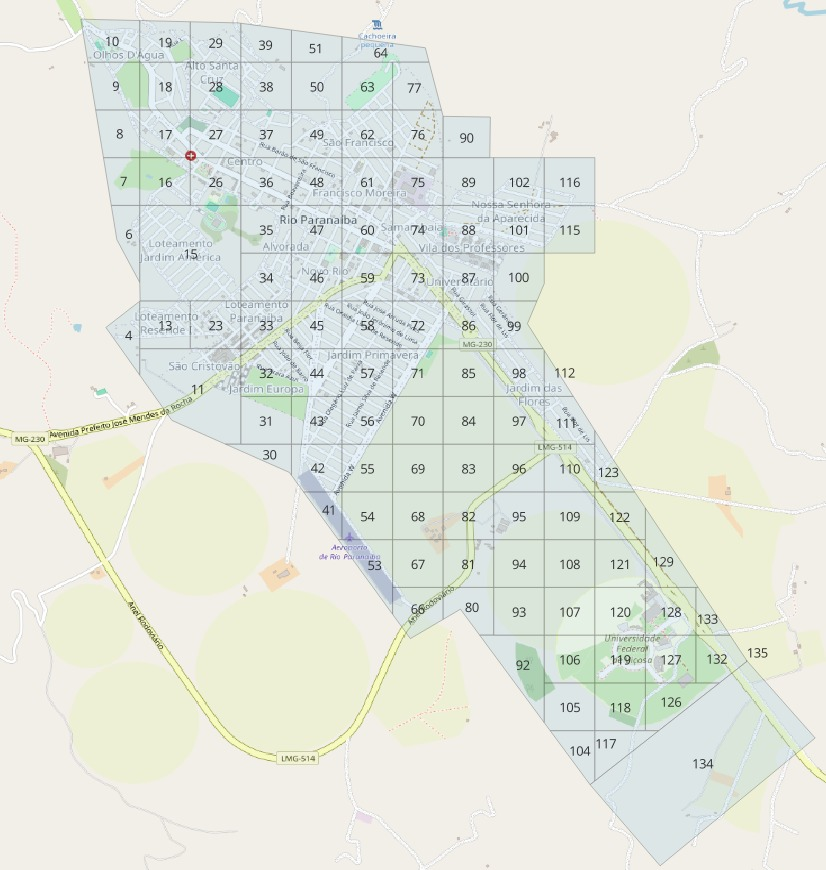
\includegraphics[width=\textwidth]{setorizaçãoRP.jpg}
    \caption{setorização de Rio Paranaíba}
    \label{fig:setorização}
\end{figure}

\section{Processamento de Imagens}
    As imagens coletadas serão pré-processadas para remoção de ruídos e distorções atmosféricas usando métodos de correção radiométrica, seguidos por três etapas principais de processamento: filtragem espacial com operadores de convolução para suavizar e detectar bordas, filtragem no domínio da frequência com a Transformada de Fourier para remover distorções periódicas, e binarização para segmentação dos objetos de interesse, complementada por operações morfológicas para refinar as formas detectadas.

\section{Segmentação e Classificação}
    As imagens coletadas serão pré-processadas para remoção de ruídos e distorções atmosféricas usando métodos de correção radiométrica, seguidos por três etapas principais de processamento: (1) filtragem espacial, (2) filtragem no domínio da frequência, e (3) binarização e operações morfológicas para segmentação e refinamento dos objetos de interesse.

\subsection{Filtragem Espacial}
    A filtragem espacial será realizada aplicando operadores de convolução sobre regiões 3x3 da imagem, visando suavizar e detectar bordas importantes nas imagens. Essa abordagem pode mitigar ruídos indesejados, permitindo a identificação precisa dos contornos das árvores, especialmente suas copas.

\subsection{Filtragem no Domínio da Frequência}
    Para melhorar a definição dos objetos, será aplicada a Transformada de Fourier, que permitiu a remoção de distorções periódicas e artefatos de baixa frequência. Esse método resulta em uma definição mais clara das estruturas relevantes das árvores, como as copas e troncos, aprimorando o contraste e a distinção dos elementos presentes nas imagens.

\subsection{Binarização e Operações Morfológicas}
    Após a filtragem, as imagens serão submetidas a técnicas de binarização, como o método de Otsu, para segmentação dos objetos de interesse. Essa binarização transforma as imagens em um formato binário (preto e branco) onde as árvores serão destacadas em relação ao fundo. A segmentação pode ser refinada com operações morfológicas, como a dilatação e erosão, que diminuem ruídos menores e conectaram componentes disjuntos, melhorando a continuidade das formas detectadas.
%fluxograma

\section{Ferramentas e Softwares}
    Os principais softwares e ferramentas são discutidos nesta parte do relatório, que serão adotados para a fase de pré-processamento de dados, a fim de preparar as imagens e informações coletadas para que possam ser efetivamente processadas pelas técnicas de detecção e classificação de falhas. As ferramentas são de grande importância para limpar e processar imagens brutas, corrigindo e fundindo os dados geoespaciais.

\subsection{TensorFlow}
   TensorFlow é uma das principais bibliotecas de aprendizado profundo amplamente utilizadas no desenvolvimento e treinamento de redes neurais artificiais. No pré-processamento, essa biblioteca será utilizada para preparar os dados de treinamento, o que inclui a normalização das imagens, redimensionamento e ajustes de contraste, além de manipular grandes conjuntos de dados de imagens. Ela também oferecem suporte para a criação de pipelines de dados eficientes, permitindo o carregamento em lote e o processamento paralelo dos dados.

\subsection{OpenCV}
    OpenCV (Open Source Computer Vision Library) é uma biblioteca de visão computacional amplamente usada para o processamento de imagens. No contexto do pré-processamento, OpenCV será fundamental para a aplicação de diversas técnicas, como:
    
    Correção de distorções: Corrigir distorções geométricas nas imagens capturadas pelos drones.
    Ajustes de cores: Realizar ajustes de brilho, contraste e balanceamento de cores, tornando os dados mais uniformes.
    Filtragem e suavização: Aplicação de filtros para remover ruídos indesejados nas imagens.
    Segmentação inicial: Realizar segmentações preliminares, como destacar áreas de interesse (copas de árvores) nas imagens para facilitar o processamento posterior.
    
\subsection{QGIS}
    QGIS (Quantum GIS) é um software de Sistema de Informação Geográfica (SIG) de código aberto, utilizado para visualização, edição e análise de dados geoespaciais. No pré-processamento, o QGIS desempenhará um papel fundamental no:
    
    Georreferenciamento: Ajustar e alinhar as imagens capturadas pelos drones com coordenadas espaciais precisas, garantindo que os dados estejam corretamente posicionados no espaço geográfico.
    Integração de dados: Combinar imagens e camadas de dados geoespaciais, como Modelos Digitais de Elevação (DEM), mapas topográficos e camadas de uso do solo, proporcionando um contexto mais rico para a análise.
    Correção atmosférica: Aplicar correções atmosféricas nas imagens de satélite, removendo interferências causadas pela atmosfera e garantindo que os dados estejam prontos para análise.
    QGIS será essencial para organizar e processar os dados geoespaciais, preparando-os para serem analisados nos próximos estágios do projeto.
    
\subsection{Keras}
    Keras é uma poderosa biblioteca de alto nível para a construção e treinamento de redes neurais em Python, integrada ao TensorFlow. Com uma interface intuitiva, Keras facilita o desenvolvimento de modelos de deep learning complexos, tornando-se uma escolha ideal para projetos que envolvem visão computacional, como a detecção e classificação de árvores. A principal vantagem do Keras é sua capacidade de permitir a construção de modelos de redes neurais convolucionais (CNNs) de maneira eficiente, permitindo que pesquisadores e desenvolvedores se concentrem no design dos modelos sem se preocupar com detalhes de implementação de baixo nível.
    
    \subsection{OpenStreetMap}
   O \textit{OpenStreetMap} (OSM) é uma plataforma colaborativa que fornece uma base de dados geoespaciais de código aberto, alimentada por contribuições voluntárias de mapeadores ao redor do mundo. Por meio de APIs como a Overpass API, é possível extrair informações detalhadas sobre árvores mapeadas em nível de rua. Esses dados, gerados pela comunidade, oferecem a possibilidade de identificar com precisão a localização de árvores individuais ou grupos de árvores em áreas urbanas. A integração dessas informações com algoritmos de visão computacional e imagens capturadas por drones pode aprimorar significativamente a classificação de árvores, proporcionando uma visão mais precisa da vegetação urbana.

    \begin{figure}[H]
        \centering
        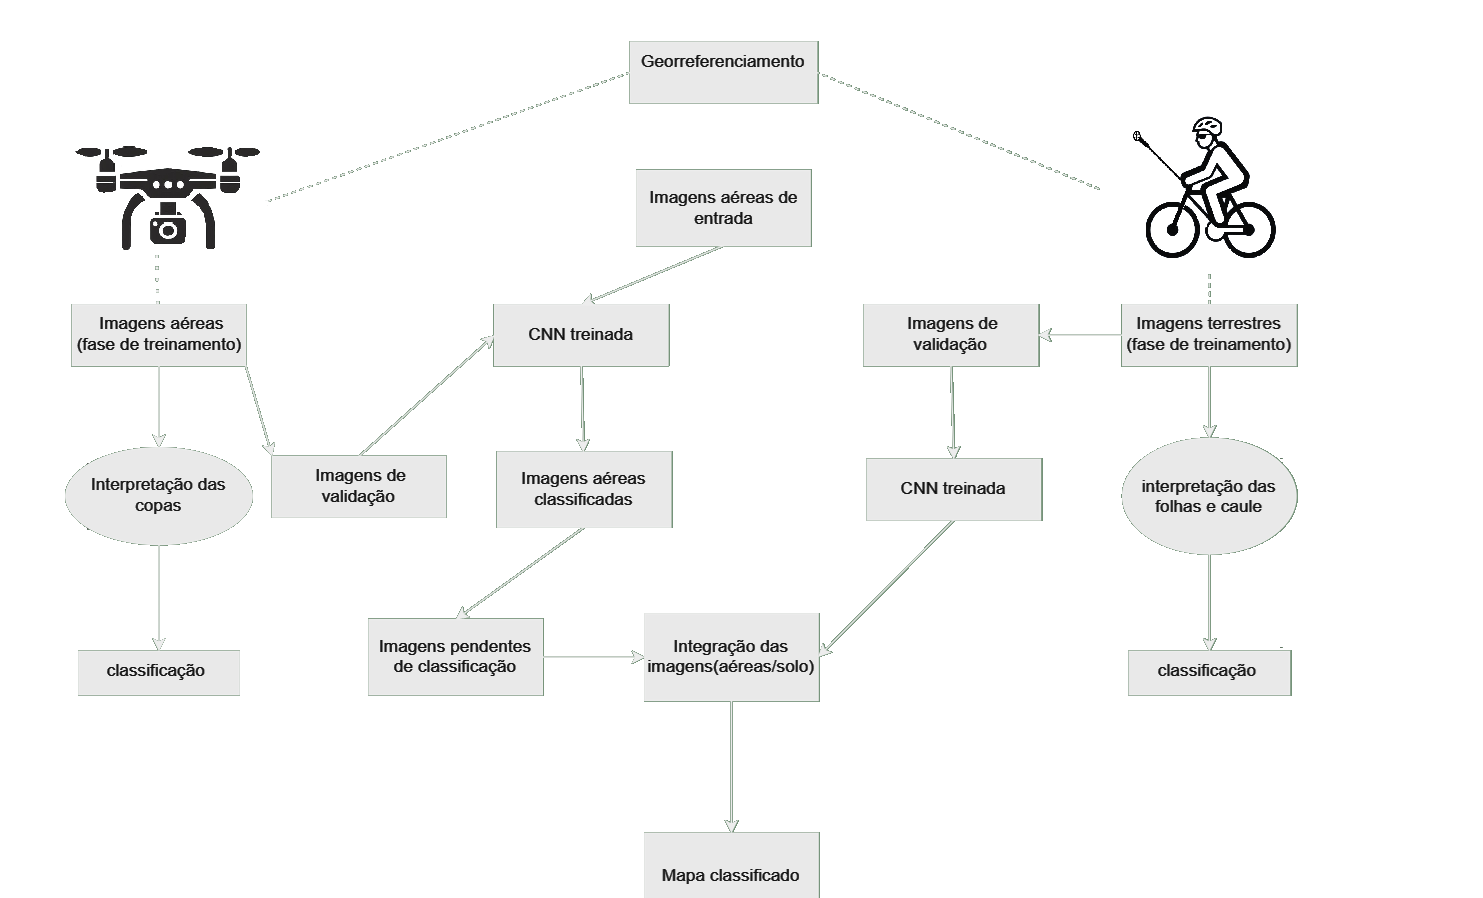
\includegraphics[width=\textwidth]{fluxograma.png}
        \caption{Etapas do projeto}
        \label{fig:Pipeline}
    \end{figure}
        
\section{Avaliação dos Resultados}
    A avaliação dos resultados será realizada com base em uma série de métricas quantitativas e qualitativas, focadas na precisão, consistência e eficiência dos dados gerados pelo modelo de detecção de árvores. Os principais aspectos a serem considerados na avaliação incluem:

    Precisão na Detecção de Árvores: A acurácia do modelo será avaliada comparando as árvores detectadas automaticamente com um conjunto de dados de referência (ground truth). A métrica de acurácia será obtida por meio da comparação entre as previsões corretas (verdadeiros positivos) e os erros (falsos positivos e falsos negativos).
\begin{equation}
    \text{Precisão} = \frac{\text{Verdadeiros Positivos (TP)}}{\text{Verdadeiros Positivos (TP)} + \text{Falsos Positivos (FP)}}
\end{equation}
    
    Taxa de Falsos Positivos e Falsos Negativos: Será calculada a taxa de falsos positivos (objetos incorretamente identificados como árvores) e de falsos negativos (árvores presentes nas imagens, mas não detectadas pelos modelos). Essas taxas ajudarão a avaliar o balanceamento entre sensibilidade e especificidade dos modelos. Posteriormente, será gerada uma matriz de confusão para avaliar o desempenho geral do modelo, permitindo a análise detalhada das classificações corretas e incorretas, além de oferecer \textit{insights} sobre o comportamento do modelo em relação à precisão e recall.
\begin{equation}
    \text{Recall} = \frac{\text{Verdadeiros Positivos (TP)}}{\text{Verdadeiros Positivos (TP)} + \text{Falsos Negativos (FN)}}
\end{equation}
    
    Eficiência Computacional: O desempenho do modelo será analisado em termos de tempo de processamento e consumo de recursos computacionais. A eficiência será um critério importante, especialmente para a aplicação em larga escala, onde o processamento rápido e otimizado é essencial.
    
    Comparação com Outras Fontes de Dados: Os resultados obtidos serão comparados com dados obtidos por outros meios, como imagens aéreas de drones e dados geoespaciais. A capacidade de integração de diferentes fontes de dados será avaliada, garantindo que o modelo seja robusto e capaz de combinar informações de diferentes perspectivas (aéreas e terrestres).
    
    Robustez do Modelo em Diferentes Cenários: A eficácia do modelo será avaliada em diferentes tipos de ambiente, incluindo áreas urbanas e rurais. Serão considerados aspectos como a densidade arbórea, variações nas condições de iluminação e a complexidade do cenário (presença de obstáculos visuais, como edifícios ou veículos).

% ============================================================
% CAPÍTULO: RESULTADOS
% ============================================================

\chapter{Resultados}\label{sec:resultados}

Este capítulo apresenta os resultados obtidos em cada etapa do sistema desenvolvido: a segmentação binária das copas de árvores com a U-Net, a separação de instâncias individuais via algoritmo \textit{Watershed} e a classificação de espécies arbóreas com a EfficientNet-B0. Ao final, descreve-se o produto integrado do \textit{pipeline}, composto por arquivos geoespaciais com a localização e a espécie predita de cada árvore detectada.

% ------------------------------------------------------------
\section{Configuração Experimental}\label{sec:config_exp}
% ------------------------------------------------------------

Os experimentos foram realizados em um ambiente Linux com GPU NVIDIA, utilizando as bibliotecas PyTorch 2.x e \textit{segmentation\_models\_pytorch}. As imagens aéreas, capturadas em formato GeoTIFF pelo drone sobre a cidade de Rio Paranaíba -- MG, foram recortadas em \textit{tiles} de $512 \times 512$ pixels. As máscaras binárias de referência (\textit{ground truth}) foram criadas manualmente, associando cada pixel à classe \textit{árvore} (1) ou \textit{fundo} (0).

A divisão dos dados seguiu a proporção 70\% para treinamento e 30\% para validação, com seleção aleatória fixa (\texttt{random\_state = 42}) para garantir reprodutibilidade. A função de perda utilizada no treinamento da U-Net combinou a \textit{Binary Cross-Entropy} (BCE) e a \textit{Dice Loss} em partes iguais:

\begin{equation}
    \mathcal{L} = 0{,}5 \cdot \mathcal{L}_{\text{BCE}} + 0{,}5 \cdot \mathcal{L}_{\text{Dice}}
    \label{eq:loss}
\end{equation}

Essa combinação tem como objetivo equilibrar a sensibilidade a falsos negativos (Dice) com a estabilidade numérica do treinamento (BCE) \cite{jadon2020survey}. O otimizador AdamW foi empregado com \textit{weight decay} de $10^{-4}$, e o treinamento utilizou precisão mista (\textit{Automatic Mixed Precision} -- AMP) para reduzir o consumo de memória e acelerar os cálculos.

% ------------------------------------------------------------
\section{Segmentação Binária de Copas de Árvores}\label{sec:result_seg}
% ------------------------------------------------------------

A segmentação das copas de árvores nas imagens aéreas foi realizada por uma U-Net \cite{ronneberger2015u}, cujo codificador (\textit{encoder}) foi pré-treinado no conjunto ImageNet. Foram conduzidos dois conjuntos de experimentos: primeiro, uma comparação entre diferentes arquiteturas de \textit{encoder} para selecionar a mais adequada à tarefa; segundo, uma análise do impacto da resolução das imagens e das estratégias de aumento de dados (\textit{data augmentation}).

% - - - - - - - - - - - - - - - - - - - - - - - - - - - - - -
\subsection{Comparativo de Encoders}\label{sec:bench_enc}
% - - - - - - - - - - - - - - - - - - - - - - - - - - - - - -

Quatro arquiteturas de \textit{encoder} foram avaliadas em duas taxas de aprendizado distintas ($10^{-4}$ e $5 \times 10^{-5}$), mantendo os demais hiperparâmetros fixos: imagens de $512 \times 512$ pixels, \textit{batch size} de 6 e até 40 épocas com \textit{early stopping} (paciência de 5 épocas). A métrica de referência adotada foi o \textit{Intersection over Union} (IoU), também denominada Índice de Jaccard:

\begin{equation}
    \text{IoU} = \frac{|A \cap B|}{|A \cup B|} = \frac{TP}{TP + FP + FN}
    \label{eq:iou}
\end{equation}

A Tabela~\ref{tab:benchmark_encoders} apresenta o melhor IoU obtido por cada configuração no conjunto de validação.

\begin{table}[H]
    \centering
    \caption[Comparativo de encoders da U-Net]{Comparativo entre encoders para a U-Net na tarefa de segmentação binária de copas. Melhor IoU de validação por configuração de \textit{encoder} e taxa de aprendizado.}
    \label{tab:benchmark_encoders}
    \begin{tabular}{llcc}
        \toprule
        \textbf{Encoder}         & \textbf{Taxa de Aprendizado} & \textbf{Melhor IoU} & \textbf{Limiar ótimo} \\
        \midrule
        ResNet-34                & $1{,}0 \times 10^{-4}$       & 0,706               & 0,6 \\
        ResNet-34                & $5{,}0 \times 10^{-5}$       & 0,706               & 0,6 \\
        ResNet-50                & $1{,}0 \times 10^{-4}$       & 0,717               & 0,5 \\
        ResNet-50                & $5{,}0 \times 10^{-5}$       & 0,706               & 0,6 \\
        MobileNet-V2             & $1{,}0 \times 10^{-4}$       & 0,718               & 0,5 \\
        MobileNet-V2             & $5{,}0 \times 10^{-5}$       & 0,713               & 0,6 \\
        EfficientNet-B0          & $1{,}0 \times 10^{-4}$       & 0,719               & 0,7 \\
        \textbf{EfficientNet-B0} & $\mathbf{5{,}0 \times 10^{-5}}$ & \textbf{0,722}  & \textbf{0,5} \\
        \bottomrule
    \end{tabular}
    \fonte{Próprio Autor}
\end{table}

A EfficientNet-B0 com taxa de aprendizado $5 \times 10^{-5}$ obteve o melhor desempenho, alcançando IoU de $0{,}722$ com limiar de binarização de $0{,}5$. A ResNet-34 apresentou os resultados mais baixos nas duas taxas testadas ($\text{IoU} = 0{,}706$), enquanto ResNet-50 e MobileNet-V2 ficaram em posição intermediária. Apesar das diferenças absolutas serem pequenas (menos de 2 pontos percentuais), a EfficientNet-B0 demonstrou melhor equilíbrio entre capacidade representacional e custo computacional, justificando sua adoção para experimentos subsequentes de classificação de espécies.

% - - - - - - - - - - - - - - - - - - - - - - - - - - - - - -
\subsection{Impacto da Resolução e do Aumento de Dados}\label{sec:res_aug}
% - - - - - - - - - - - - - - - - - - - - - - - - - - - - - -

Além do \textit{encoder}, investigou-se o efeito da resolução das imagens de entrada e da aplicação de \textit{data augmentation} suave sobre o desempenho de segmentação. Foram realizados três experimentos principais com o \textit{encoder} ResNet-34, conforme descrito na Tabela~\ref{tab:res_aug}.

\begin{table}[H]
    \centering
    \caption[Impacto da resolução e augmentation na segmentação]{Efeito da resolução e do aumento de dados no desempenho da U-Net (encoder ResNet-34). Métricas reportadas na melhor época do conjunto de validação.}
    \label{tab:res_aug}
    \begin{tabular}{lccccc}
        \toprule
        \textbf{Configuração}         & \textbf{Res.} & \textbf{Melhor IoU} & \textbf{F1} & \textbf{Precisão} & \textbf{Recall} \\
        \midrule
        Sem augmentation              & 256 px & 0,750 & 0,857 & 0,829 & 0,888 \\
        Com aug. suave (softAug)      & 256 px & 0,722 & 0,838 & 0,809 & 0,870 \\
        \textbf{Com aug. suave (softAug)} & \textbf{512 px} & \textbf{0,749} & \textbf{0,857} & \textbf{0,831} & \textbf{0,884} \\
        Com aug. suave (softAug) -- run 2 & 512 px & 0,745 & 0,854 & 0,832 & 0,877 \\
        \bottomrule
    \end{tabular}
    \fonte{Próprio Autor}
\end{table}

As estratégias de \textit{data augmentation} empregadas foram conservadoras (\textit{softAug}): recorte aleatório com escala entre 85\% e 100\% da imagem (\texttt{RandomResizedCrop}), espelhamento horizontal com probabilidade de 50\%, e perturbações de brilho, contraste e saturação com variação de 5\% (\texttt{ColorJitter}). Optou-se por augmentações suaves porque perturbações agressivas em imagens aéreas de copas de árvores tendem a distorcer padrões de textura e forma que são discriminativos para a tarefa.

Os resultados mostram que a resolução de $512 \times 512$ pixels com augmentation suave atingiu desempenho equiparável à configuração sem augmentation em $256 \times 256$ pixels (IoU de $0{,}749$ vs. $0{,}750$), ao mesmo tempo em que contribui para maior capacidade de generalização do modelo. A aplicação de augmentation em resolução $256 \times 256$ resultou em queda de desempenho (IoU = $0{,}722$), possivelmente pelo fato de que o recorte aleatório em imagens menores elimina informações estruturais relevantes das copas.

% - - - - - - - - - - - - - - - - - - - - - - - - - - - - - -
\subsection{Evolução do Treinamento}\label{sec:curvas}
% - - - - - - - - - - - - - - - - - - - - - - - - - - - - - -

A Figura~\ref{fig:curvas_seg} apresenta as curvas de perda, F1-Score e IoU ao longo das épocas de treinamento para o melhor modelo de segmentação (ResNet-34, $512 \times 512$ px, aug. suave, $\text{lr} = 10^{-4}$). O modelo atingiu seu pico de desempenho na época 17, com IoU de $0{,}749$, precisão de $0{,}831$, \textit{recall} de $0{,}884$ e F1-Score de $0{,}857$ no conjunto de validação. A partir dessa época, observa-se estabilização das métricas de validação, sem ganhos adicionais significativos, indicando convergência adequada do treinamento.

\begin{figure}[H]
    \centering
    % INSTRUÇÃO: gerar este gráfico com matplotlib a partir de unet_metrics_512_softAug.csv
    % Sugestão: duas subplots — (1) train_loss vs val_loss por época; (2) f1 e iou por época
    \includegraphics[width=\textwidth]{curvas_treinamento_seg.png}
    \caption[Curvas de treinamento do modelo de segmentação]{Evolução das métricas durante o treinamento do melhor modelo de segmentação (U-Net ResNet-34, $512 \times 512$ px). Acima: perdas de treino e validação. Abaixo: F1-Score e IoU de validação por época.}
    \label{fig:curvas_seg}
\end{figure}

O escalonamento automático da taxa de aprendizado (\texttt{ReduceLROnPlateau}, paciência = 3, fator = 0,5) contribuiu para a estabilidade do treinamento ao reduzir a taxa quando o IoU de validação não apresentava melhora por três épocas consecutivas. O \textit{early stopping} com paciência de 5 épocas impediu o sobreajuste nas fases finais do treinamento.

% ------------------------------------------------------------
\section{Separação de Instâncias com Watershed}\label{sec:result_watershed}
% ------------------------------------------------------------

A máscara binária produzida pela U-Net representa a área de cobertura de copa de forma agregada, sem distinguir copas individuais que se tocam ou se sobrepõem. Para individualizar cada árvore, aplicou-se o algoritmo \textit{Watershed} baseado em transformada de distância, conforme descrito a seguir.

Cada máscara binária predita passou por um pré-processamento morfológico: fechamento com disco de raio 5 pixels (\texttt{disk(5)}), remoção de pequenos buracos (limiar de área = 32 px$^2$) e remoção de objetos muito pequenos (tamanho mínimo = 32 px$^2$). Em seguida, calculou-se a transformada de distância euclidiana sobre a máscara limpa e identificaram-se os máximos locais com \textit{footprint} de $15 \times 15$ pixels como marcadores de centroide. O \textit{Watershed} foi então aplicado usando esses marcadores como sementes, delimitando regiões individuais de copa. Instâncias com área inferior a 150 pixels foram descartadas como ruído.

A Figura~\ref{fig:watershed} ilustra o processo de separação de instâncias em uma \textit{tile} de exemplo, desde a máscara binária predita até a máscara de instâncias rotuladas.

\begin{figure}[H]
    \centering
    % INSTRUÇÃO: inserir imagem comparando tile original, máscara binária e máscara de instâncias
    \includegraphics[width=\textwidth]{watershed_exemplo.png}
    \caption[Separação de instâncias com Watershed]{Exemplo de separação de copas individuais via \textit{Watershed}. Da esquerda para a direita: imagem aérea original, máscara binária predita pela U-Net e máscara de instâncias individuais após segmentação por \textit{Watershed}.}
    \label{fig:watershed}
\end{figure}

% ------------------------------------------------------------
\section{Classificação de Espécies Arbóreas}\label{sec:result_cls}
% ------------------------------------------------------------

Para cada instância de copa detectada e individualizada, extraiu-se um recorte (\textit{crop}) da imagem aérea original com margem de 16 pixels ao redor da bounding box da instância, redimensionado para $512 \times 512$ pixels. Esses recortes foram classificados por uma EfficientNet-B0 \cite{tan2019efficientnet} pré-treinada no ImageNet e ajustada para a tarefa de classificação de 6 espécies arbóreas (\textit{fine-tuning}).

O conjunto de dados de classificação foi composto por recortes anotados manualmente e por pseudorrótulos gerados automaticamente pelo próprio \textit{pipeline} (recortes com confiança de classificação superior a 0,5). Para mitigar o desbalanceamento de classes, o conjunto foi balanceado por aumento de dados (\texttt{augment\_rare\_species.py}), atingindo até 1.200 amostras para a espécie predominante e 800 amostras para cada uma das demais 5 espécies. Adicionalmente, o \texttt{WeightedRandomSampler} do PyTorch foi utilizado durante o treinamento para garantir amostragem equilibrada entre as classes a cada época.

O treinamento utilizou os seguintes hiperparâmetros: otimizador AdamW ($\text{lr} = 10^{-4}$, \textit{weight decay} = $10^{-4}$), função de perda \textit{CrossEntropyLoss}, escalonador co-ssenoidal (\texttt{CosineAnnealingLR}, $T_{\max} = 10$) e \textit{early stopping} com paciência de 5 épocas, com seleção do melhor modelo pelo F1-Score macro no conjunto de validação (divisão 80\%/20\%, estratificada por espécie).

A Tabela~\ref{tab:result_cls} apresenta as métricas obtidas pelo melhor modelo de classificação no conjunto de validação.

\begin{table}[H]
    \centering
    \caption[Métricas do classificador de espécies EfficientNet-B0]{Desempenho do classificador de espécies arbóreas (EfficientNet-B0) no conjunto de validação. Métricas calculadas com média macro entre as 6 classes.}
    \label{tab:result_cls}
    \begin{tabular}{lc}
        \toprule
        \textbf{Métrica}    & \textbf{Valor} \\
        \midrule
        Acurácia            & % TODO: preencher com o valor real do log de treinamento \\
        F1-Score (macro)    & % TODO: preencher com o valor real do log de treinamento \\
        \bottomrule
    \end{tabular}
    \fonte{Próprio Autor}
\end{table}

% INSTRUÇÃO: substituir os % TODO acima pelos valores reais obtidos no terminal ao rodar
% train_species_efficientnet.py. A saída final imprime:
%   "Melhor F1 obtido: X.XXXX"
% Adicionar também a matriz de confusão como figura, se disponível.

A Figura~\ref{fig:matriz_confusao} apresenta a matriz de confusão do classificador, evidenciando as espécies com maior taxa de acerto e aquelas com maior confusão entre classes.

\begin{figure}[H]
    \centering
    % INSTRUÇÃO: gerar a matriz de confusão durante a avaliação do modelo e exportar como imagem
    \includegraphics[width=0.75\textwidth]{matriz_confusao_especies.png}
    \caption[Matriz de confusão do classificador de espécies]{Matriz de confusão do classificador EfficientNet-B0 no conjunto de validação para as 6 espécies arbóreas identificadas em Rio Paranaíba -- MG.}
    \label{fig:matriz_confusao}
\end{figure}

% ------------------------------------------------------------
\section{Pipeline Integrado e Saída Geoespacial}\label{sec:result_pipeline}
% ------------------------------------------------------------

O \textit{pipeline} completo integrou as etapas de segmentação (U-Net), separação de instâncias (\textit{Watershed}) e classificação de espécies (EfficientNet-B0), gerando como produto final arquivos geoespaciais nos formatos GeoPackage (.gpkg) e GeoJSON. Cada instância de árvore detectada é representada como um polígono georeferenciado com os seguintes atributos: espécie predita (\texttt{predicted\_species}), confiança da predição (\texttt{confidence}), área da copa em metros quadrados (\texttt{area\_m2}), \textit{tile} de origem (\texttt{tile}) e identificador da instância (\texttt{instance\_id}).

Para lidar com instâncias duplicadas geradas em regiões de sobreposição entre \textit{tiles} adjacentes, aplicou-se o algoritmo DBSCAN sobre as coordenadas centroides das instâncias. Instâncias a menos de 2 metros entre si foram agrupadas e representadas por uma única entrada no arquivo de saída, mantendo a predição de maior confiança.

A Figura~\ref{fig:mapa_resultado} apresenta uma visualização dos resultados no ambiente QGIS, exibindo as copas segmentadas e classificadas sobre a ortofoto da área urbana de Rio Paranaíba.

\begin{figure}[H]
    \centering
    % INSTRUÇÃO: exportar visualização do GeoPackage no QGIS com legenda de espécies
    \includegraphics[width=\textwidth]{mapa_resultado_especies.png}
    \caption[Mapa de árvores detectadas e classificadas em Rio Paranaíba]{Resultado do \textit{pipeline} de detecção e classificação de árvores urbanas sobre a ortofoto de Rio Paranaíba -- MG. Cada polígono representa uma copa detectada, com cor correspondente à espécie predita pelo modelo.}
    \label{fig:mapa_resultado}
\end{figure}


%     \chapter{Resultados Esperados}\label{sec:resultEsperados}
%     O foco principal deste projeto é projetar um sistema integrado que possa integrar imagens de árvores ao nível da rua, obtidas pelo OpenStreetMap, com imagens de árvores capturadas por drones em um mesmo conjunto de dados de treinamento, para apoiar a classificação de espécies de árvores tanto em ambientes urbanos quanto rurais. Desse modo, o seguinte deve ser feito:
    
%     Classificação Melhorada de Árvores: Com a fusão das imagens colhidas ao nível do solo e das imagens de drones capturadas do ar, o modelo que está sendo treinado deve ser mais capaz de classificar e identificar as espécies arbóreas. As fotos de nível da rua podem oferecer informações qualitativas e altamente descritivas em termos da espécie da árvore, forma, cor e características distintivas das folhas, cascas e coroas, complementando as fotos aéreas.
    
%     Melhor Precisão na Identificação de Espécies: A disponibilidade de imagens terrestres e aéreas aumentará maciçamente a precisão do modelo na identificação de espécies, especialmente em áreas com densidade de vegetação e complexidade urbana. O sistema poderá identificar espécies específicas com características semelhantes que não podem ser identificadas apenas por imagens aéreas.
    
%     Desenvolvimento de uma Ferramenta Universal para Diferentes Aplicações: A ferramenta a ser desenvolvida terá várias aplicações práticas na ecologia, no planejamento urbano, no monitoramento ambiental, bem como na gestão de recursos naturais. Ela fornecerá informações precisas sobre biodiversidade, ajudará no planejamento e gerenciamento de árvores e facilitará o monitoramento de mudanças ambientais.
    
%     Robustez na Detecção em Diversos Ambientes: O modelo será robusto em ambientes urbanos, rurais e naturais. A combinação de dados aéreos e terrestres permitirá análises em situações onde os dados puramente aéreos seriam limitados, como áreas com densa vegetação ou obstruções visuais.
    
%     Melhoria do Monitoramento Ambiental e Gestão de Recursos Naturais: A solução permitirá monitorar a saúde das árvores, detectar danos ao ecossistema e apoiar a gestão de florestas urbanas e rurais, com insights automatizados e em tempo real sobre o estado das árvores.
    
%     Eficiência na Coleta e Processamento de Dados: O sistema automatizará grande parte do processo de coleta, anotação e análise de dados, resultando em maior eficiência e escalabilidade para grandes projetos com monitoramento em tempo real.
    

% \chapter{Cronograma}\label{sec:cronograma}


% \begin{table}[htbp]
%   \centering
%   \caption[Cronograma Normal]{Cronograma do Projeto em Meses}
%   \label{tab:cronograma}
%   \begin{tabular}{lcccccc}
%     \toprule
%     \textbf{Atividade} & \textbf{1} & \textbf{2} & \textbf{3} & \textbf{4} & \textbf{5} & \textbf{6} \\
%     \midrule
%     Revisão Bibliográfica & $\bullet$ & $\bullet$ & $\bullet$ & & & \\
%     Coleta de Dados Aéreos & & & $\bullet$ & $\bullet$ & & \\
%     Coleta de Dados Terrestres & & & $\bullet$ & $\bullet$ & & \\
%     Processamento de Imagens & & & & $\bullet$ & $\bullet$ & \\
%     Segmentação e Classificação & & & & & $\bullet$ & \\
%     Resultados e Avaliação & & & & & $\bullet$ & $\bullet$ \\
%     Conclusão & & & & & & $\bullet$ \\
%     Banca & & & & & & $\bullet$ \\
%     \bottomrule
%   \end{tabular}
%   \fonte{Próprio Autor}
% \end{table}




% ----------------------------------------------------------
% ELEMENTOS PÓS-TEXTUAIS
% ----------------------------------------------------------
\postextual

% Referências bibliográficas

%\bibliography{referencias}
\linespread{1}
\printbibliography
% Caso sejam necessários apêndices ou anexos em seu documento
% Use os ambientes abaixo

%% Apêndices
%
%% Inicia os apêndices
%\begin{apendicesenv}
%
%% Imprime uma página indicando o início dos apêndices
%\partapendices
%
%\chapter{Primeiro Apêndice}
%
%\chapter{Segundo Apêndice}
%
%\end{apendicesenv}
%
%% ----------------------------------------------------------
%% Anexos
%% ----------------------------------------------------------
%\begin{anexosenv}
%
%% Imprime uma página indicando o início dos anexos
%\partanexos
%
%\chapter{Primeiro Anexo}
%\lipsum[30]
%
%\chapter{Segundo Anexo}
%\lipsum[31]
%
%\end{anexosenv}

\end{document}
